\section{Intrinsically Photosensitive Retinal Ganglion Cells (ipRGCs)}

\textit{Recent reviews by \citet{spitschan_melanopsin_2019} and \citet{do_melanopsin_2019} provide authoritative overviews of this rapidly progressing research area.}

\bigskip

Retinal rod and cone cells (of three types, l/m/s) are well established as the primary receptors for human vision, and their connections and properties are relatively well understood. Two distinct signalling pathways originate from the retina, one of which is associated with image formation and the other which is considered to be \gls{NIF}, and which influences systems such as circadian rhythm entrainment, pupillary reflex and melatonin release. It was originally thought that rods and cones were the sole inputs to both of these pathways \citep{hankins_melanopsin_2008}.

\Glspl{RGC} combine signals from groups of cones and rods and relay these signals via the optic nerve to the lateral geniculate nucleus, which in turn processes and relays them further to the cortex for additional processing, allowing for classical vision of objects, movement and colour. \Glspl{ipRGC} are a sub-class of \glspl{RGC}, which in addition to combining and relaying signals exhibit some intrinsic photosensitivity of their own. 

This intrinsic photosenstivity was only confirmed recently relative to our knowledge of other retinal cell types \citep{qiu_induction_2005}, following a search for a retinal cell type or combination of cell types which would fit the spectral sensitivity properties found to influence entrainment of the circadian rhythm in humans and other animals \citep{brainard_human_2001,brainard_action_2001}, which was dissimilar to all of the spectral sensitivities of the cell classes known at the time.

Additionally, it was found that animals and humans with no functioning rods or cones were still able to have a correctly functioning circadian system \citep{freedman_regulation_1999,zaidi_short-wavelength_2007}, further suggesting that that the circadian rhythm was influenced by a novel receptor with a distinct photoreceptor. It is now believed to be these cells which provide input to the second of the signalling pathways originating in the retina, that which controls the \gls{NIF} response to illumination.

\Glspl{ipRGC} were found to express a photopigment fitting such attributes, named melanopsin. The spectral sensitivity of melanopsin peaks around 480nm \citep{qiu_induction_2005,hankins_primary_2002,dacey_melanopsin-expressing_2005,peirson_melanopsin_2006,bailes_human_2013} which places it between the s-cone (cyanolabe photopsin) and rod cell (rhodopic rhodopsin) spectral sensitivities, see Figure \ref{fig:specsens}. In humans, pre-receptoral filtering leads to a functional peak sensitivity of closer to 490nm \citep{cie_cie_2015-1}. 

Exogenously expressed mouse melanopsin has been shown to be tristable \citep{emanuel_melanopsin_2015,matsuyama_photochemical_2012-1}, that is: existing in one of three possible states. A photon interaction converts melanopsin in one of these states to another, with two of the states being electrically silent (not providing a signal) and one being signal-producing. Notably, these different states have slightly different spectral sensitivities, and thus exposure to specific wavelengths biases the population distribution in different ways, as shown in Figure \ref{fig:melssf}.

\begin{figure}[htbp]
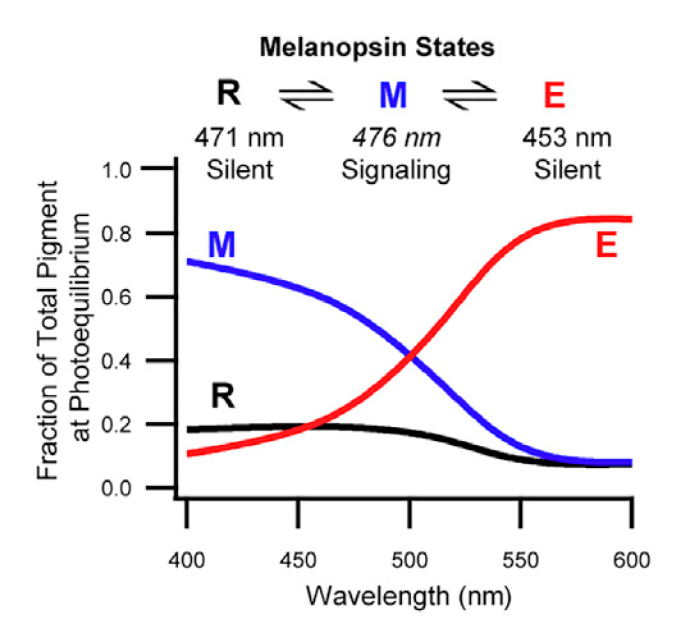
\includegraphics[max width=\textwidth, center]{figs/LitRev/melstates.png}
\caption{Reproduced from \citep{do_melanopsin_2019} (Fig 5D in original source). \textit{``[M]ouse melanopsin is understood to have three states (R, M, and E). The peak spectral sensitivities of R and E are determined from the electrophysiological responses of M1s. Spectrophotometric measurements of purified melanopsin yielded similar values (467 and 446 nm, respectively) and gave information for M (476 nm; [\citet{matsuyama_photochemical_2012-1}]). Bottom, the distribution of melanopsin states as a function of wavelength, estimated from a model based on values from purified melanopsin.''}}
\label{fig:melssf}
\end{figure}

Human melanopsin appears to be bistable (of two states), and there is uncertainty regarding whether this bistability would have physiological consequences \citep{cie_cie_2015-1,mure_melanopsin_2009,rollag_does_2008,wada_color_2018,mure_melanopsin-dependent_2007,mawad_absence_2008,koyanagi_cephalochordate_2005,emanuel_melanopsin_2015}.

\begin{figure}[htbp]
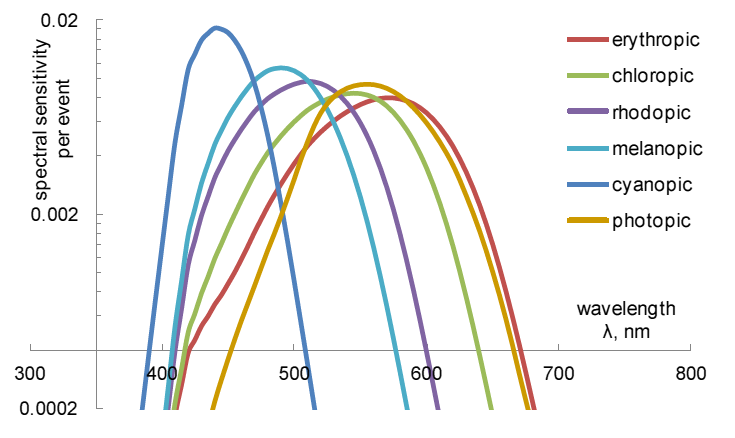
\includegraphics[max width=\textwidth, center]{figs/LitRev/ciemel.png}
\caption{Reproduced from \gls{CIE} TN 003:2015 \citep{cie_cie_2015-1}. \textit{``Spectral sensitivity curves of the five human photopigments to irradiance at the outer surface of the eye of the standard observer and photopic spectral efficiency, normalized to equal area.''}}
\label{fig:specsens}
\end{figure}

\Glspl{ipRGC} are sparse in the retina; discounting input from other cell types, they operate at a much lower resolution than as would be required for meaningful spatial vision. They also operate much more slowly compared to other cell types, taking several seconds to respond, but are able to sustain a response in contrast to other retinal cell types which are able to respond quickly but only for short periods.

It has been proposed that \glspl{ipRGC} may allow an observer to sense a level of absolute irradiance \citep{brown_melanopsin_2010}. 

\subsection{ipRGC connectivity}

\begin{figure}[htbp]
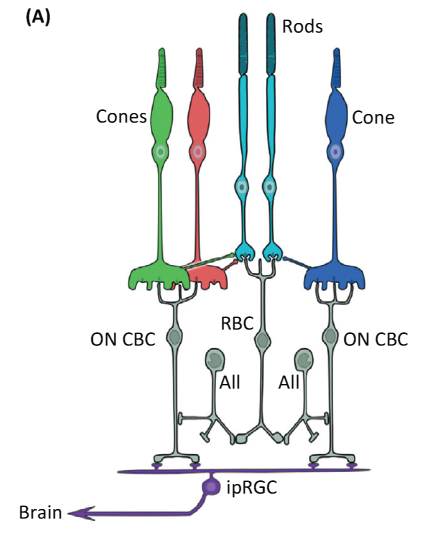
\includegraphics[max width=\textwidth, center]{figs/LitRev/lucas.png}
\caption{Reproduced from \citet{lucas_measuring_2014}. \textit{``Schematic of the relevant retinal circuitry in humans. Non-image-forming responses originate in the retina and have been attributed to a particular class of retinal ganglion cell (ipRGC). ipRGCs are directly photosensitive owing to expression of melanopsin, which allows them to respond to light even when isolated from the rest of the retina. In situ they are connected to the outer retinal rod and cone photoreceptors via the conventional retinal circuitry. The details of their intraretinal connections are not completely understood and probably vary between different subtypes. Shown here are major connections with on cone bipolar cells (on CBCs) connecting them to cone and, via amacrine cells (AII) and rod bipolar cells (RBC), rod photoreceptors. As a consequence, the firing pattern of ipRGCs can be influenced by both intrinsic melanopsin photoreception and extrinsic signals originating in rods and each of the spectrally distinct cone classes (shown in red, green, and blue). ''}}
\label{fig:lucas}
\end{figure}

\subsection{The roles of ipRGCs beyond circadian entrainment}
\label{sec:ipRGCbeyond}

In recent years there has been a number of publications examining the role of melanopsin outside of \gls{NIF} vision, challenging some of the assumptions about the abilities of signals originating from \glspl{ipRGC}.

A number of studies have found that the signals from ipRGCs are capable of encoding spatial structure \citep{ecker_melanopsin-expressing_2010, mouland_responses_2017, allen_melanopsin_2017, allen_form_2019, zhao_photoresponse_2014} (Commentary: \citet{spitschan_vision_2017,sonoda_re-evaluating_2016})
%
Additionally, several researchers have investigated whether \glspl{ipRGC} may play a role in chromatic vision \citep{cao_evidence_2018, spitschan_human_2017-1,zele_melanopsin_2018}.

\citet{spitschan_human_2017-1} used a silent substitution paradigm to target melanopsin and found an fMRI response in V1 for each of four participants, in contradiction to an earlier study by the same group \citep{spitschan_human_2016}\footnote{``we now regard our prior study as not fully resolving the possibility that rapid modulation of the ipRGCs drives a cortical response'' \citep{spitschan_human_2017-1}}. Participants reported a visual percept which was `unpleasant, blurry, minimal brightening that quickly faded'.

\citet{cao_evidence_2018} found that ``changing melanopsin activation levels shifts the equilibrium point in the chromatic pathways'', though curiously the effect was only present for the L/(L+M) pathway.

\citet{zele_melanopsin_2018} found evidence that ``putative melanopsin-mediated image-forming vision corresponds to an opponent S-OFF L+M-ON response property, with an average temporal resolution up to approximately 5 Hz, and $>$10x higher thresholds than red-green colour vision''. The key figure from \citet{zele_melanopsin_2018} is reproduced in Figure \ref{fig:zele}.

\begin{figure}[htbp]
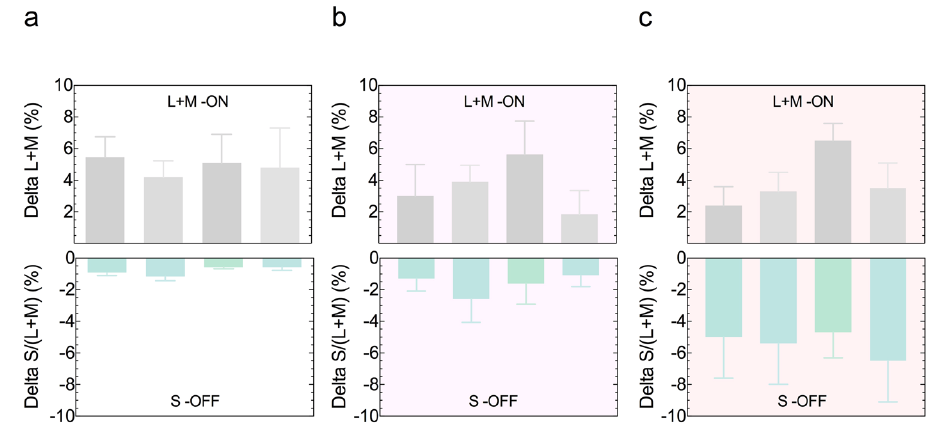
\includegraphics[max width=\textwidth, center]{figs/LitRev/zele.png}
\caption{Reproduced from \citet{zele_melanopsin_2018}. \textit{``Melanopsin photoreception is analogous to an increment in cone luminance [L + M] and a decrement in S-cone excitation [S/(L + M)] with white (a), yellowish-pink (b) and orange adapting stimulus fields (c).''}}
\label{fig:zele}
\end{figure}

Very recent results from \citet{vincent_adaptation_2019,vincent_adaptation_2019-1} report that, contrary to expectations (based on the work of \citet{allen_melanopsin-driven_2014}), ``sensitivity to flicker directed at the cones was not altered by adaptation to a steady field of substantially higher melanopic content''. 

Though these results are exciting, there are a number of methodological and theoretical areas which require development. The standard methodology used in these experiments is that of `silent substitution' \citep{estevez_silent_1982,kamar_silent-substitution_2019,spitschan_method_2018} where careful tuning of the spectrum is used (see the topic of `metameric blacks' \citep{vienot_verriest_2014,cohen_metameric_1982,vienot_domain_2012,vienot_dimensionality_2015}) to generate signals which are only visible to the chosen receptor-type in theory, in this case melanopsin-expressing \glspl{ipRGC}. However, due to variability in observer spectral sensitivities, and limits on the level of stimulus control, it is likely that there will be a small amount of unintended stimulation of non-target cell groups. \citet{spitschan_selective_2015} refer to this as `splatter' (``the expected amount of contrast on nominally silenced photoreceptor classes for a given modulation around a given background''). A suggested control condition is to generate contrast for the nominally silenced cell groups at the level predicted from modelling.

\subsubsection{Value for colour constancy}

\hl{Up-stream from photoreceptors

Absolute rather than adaptive signaling

Slow and long temporal response

Large receptive fields}



\clearpage


